\documentclass[1p]{elsarticle_modified}
%\bibliographystyle{elsarticle-num}

%\usepackage[colorlinks]{hyperref}
%\usepackage{abbrmath_seonhwa} %\Abb, \Ascr, \Acal ,\Abf, \Afrak
\usepackage{amsfonts}
\usepackage{amssymb}
\usepackage{amsmath}
\usepackage{amsthm}
\usepackage{scalefnt}
\usepackage{amsbsy}
\usepackage{kotex}
\usepackage{caption}
\usepackage{subfig}
\usepackage{color}
\usepackage{graphicx}
\usepackage{xcolor} %% white, black, red, green, blue, cyan, magenta, yellow
\usepackage{float}
\usepackage{setspace}
\usepackage{hyperref}

\usepackage{tikz}
\usetikzlibrary{arrows}

\usepackage{multirow}
\usepackage{array} % fixed length table
\usepackage{hhline}

%%%%%%%%%%%%%%%%%%%%%
\makeatletter
\renewcommand*\env@matrix[1][\arraystretch]{%
	\edef\arraystretch{#1}%
	\hskip -\arraycolsep
	\let\@ifnextchar\new@ifnextchar
	\array{*\c@MaxMatrixCols c}}
\makeatother %https://tex.stackexchange.com/questions/14071/how-can-i-increase-the-line-spacing-in-a-matrix
%%%%%%%%%%%%%%%

\usepackage[normalem]{ulem}

\newcommand{\msout}[1]{\ifmmode\text{\sout{\ensuremath{#1}}}\else\sout{#1}\fi}
%SOURCE: \msout is \stkout macro in https://tex.stackexchange.com/questions/20609/strikeout-in-math-mode

\newcommand{\cancel}[1]{
	\ifmmode
	{\color{red}\msout{#1}}
	\else
	{\color{red}\sout{#1}}
	\fi
}

\newcommand{\add}[1]{
	{\color{blue}\uwave{#1}}
}

\newcommand{\replace}[2]{
	\ifmmode
	{\color{red}\msout{#1}}{\color{blue}\uwave{#2}}
	\else
	{\color{red}\sout{#1}}{\color{blue}\uwave{#2}}
	\fi
}

\newcommand{\Sol}{\mathcal{S}} %segment
\newcommand{\D}{D} %diagram
\newcommand{\A}{\mathcal{A}} %arc


%%%%%%%%%%%%%%%%%%%%%%%%%%%%%5 test

\def\sl{\operatorname{\textup{SL}}(2,\Cbb)}
\def\psl{\operatorname{\textup{PSL}}(2,\Cbb)}
\def\quan{\mkern 1mu \triangleright \mkern 1mu}

\theoremstyle{definition}
\newtheorem{thm}{Theorem}[section]
\newtheorem{prop}[thm]{Proposition}
\newtheorem{lem}[thm]{Lemma}
\newtheorem{ques}[thm]{Question}
\newtheorem{cor}[thm]{Corollary}
\newtheorem{defn}[thm]{Definition}
\newtheorem{exam}[thm]{Example}
\newtheorem{rmk}[thm]{Remark}
\newtheorem{alg}[thm]{Algorithm}

\newcommand{\I}{\sqrt{-1}}
\begin{document}

%\begin{frontmatter}
%
%\title{Boundary parabolic representations of knots up to 8 crossings}
%
%%% Group authors per affiliation:
%\author{Yunhi Cho} 
%\address{Department of Mathematics, University of Seoul, Seoul, Korea}
%\ead{yhcho@uos.ac.kr}
%
%
%\author{Seonhwa Kim} %\fnref{s_kim}}
%\address{Center for Geometry and Physics, Institute for Basic Science, Pohang, 37673, Korea}
%\ead{ryeona17@ibs.re.kr}
%
%\author{Hyuk Kim}
%\address{Department of Mathematical Sciences, Seoul National University, Seoul 08826, Korea}
%\ead{hyukkim@snu.ac.kr}
%
%\author{Seokbeom Yoon}
%\address{Department of Mathematical Sciences, Seoul National University, Seoul, 08826,  Korea}
%\ead{sbyoon15@snu.ac.kr}
%
%\begin{abstract}
%We find all boundary parabolic representation of knots up to 8 crossings.
%
%\end{abstract}
%\begin{keyword}
%    \MSC[2010] 57M25 
%\end{keyword}
%
%\end{frontmatter}

%\linenumbers
%\tableofcontents
%
\newcommand\colored[1]{\textcolor{white}{\rule[-0.35ex]{0.8em}{1.4ex}}\kern-0.8em\color{red} #1}%
%\newcommand\colored[1]{\textcolor{white}{ #1}\kern-2.17ex	\textcolor{white}{ #1}\kern-1.81ex	\textcolor{white}{ #1}\kern-2.15ex\color{red}#1	}

{\Large $\underline{12a_{0338}~(K12a_{0338})}$}

\setlength{\tabcolsep}{10pt}
\renewcommand{\arraystretch}{1.6}
\vspace{1cm}\begin{tabular}{m{100pt}>{\centering\arraybackslash}m{274pt}}
\multirow{5}{120pt}{
	\centering
	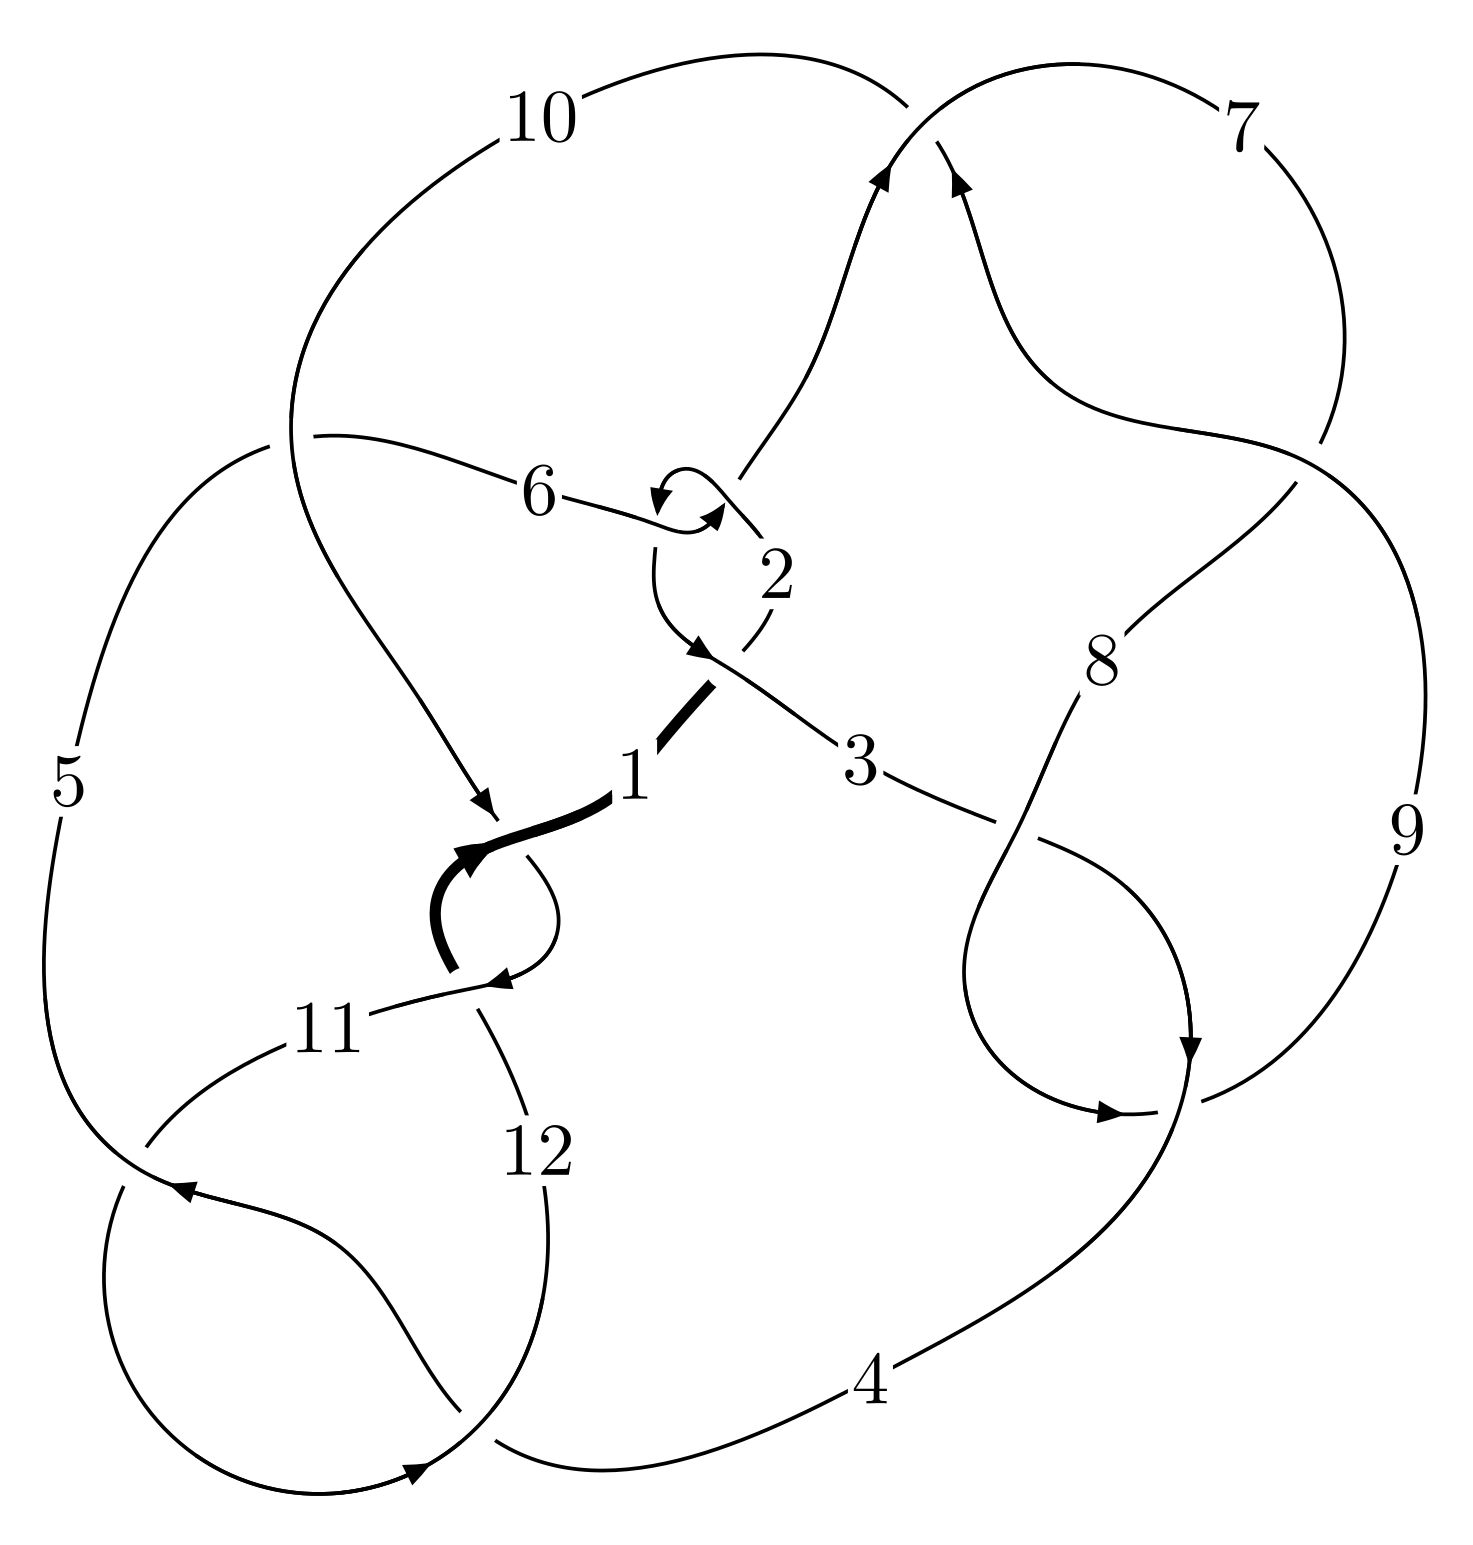
\includegraphics[width=112pt]{../../../GIT/diagram.site/Diagrams/png/1139_12a_0338.png}\\
\ \ \ A knot diagram\footnotemark}&
\allowdisplaybreaks
\textbf{Linearized knot diagam} \\
\cline{2-2}
 &
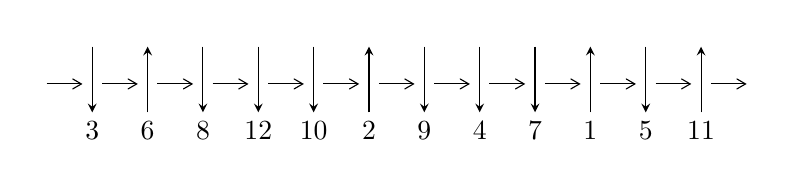
\begin{tikzpicture}[x=20pt, y=17pt]
	% nodes
	\node (C0) at (0, 0) {};
	\node (C1) at (1, 0) {};
	\node (C1U) at (1, +1) {};
	\node (C1D) at (1, -1) {3};

	\node (C2) at (2, 0) {};
	\node (C2U) at (2, +1) {};
	\node (C2D) at (2, -1) {6};

	\node (C3) at (3, 0) {};
	\node (C3U) at (3, +1) {};
	\node (C3D) at (3, -1) {8};

	\node (C4) at (4, 0) {};
	\node (C4U) at (4, +1) {};
	\node (C4D) at (4, -1) {12};

	\node (C5) at (5, 0) {};
	\node (C5U) at (5, +1) {};
	\node (C5D) at (5, -1) {10};

	\node (C6) at (6, 0) {};
	\node (C6U) at (6, +1) {};
	\node (C6D) at (6, -1) {2};

	\node (C7) at (7, 0) {};
	\node (C7U) at (7, +1) {};
	\node (C7D) at (7, -1) {9};

	\node (C8) at (8, 0) {};
	\node (C8U) at (8, +1) {};
	\node (C8D) at (8, -1) {4};

	\node (C9) at (9, 0) {};
	\node (C9U) at (9, +1) {};
	\node (C9D) at (9, -1) {7};

	\node (C10) at (10, 0) {};
	\node (C10U) at (10, +1) {};
	\node (C10D) at (10, -1) {1};

	\node (C11) at (11, 0) {};
	\node (C11U) at (11, +1) {};
	\node (C11D) at (11, -1) {5};

	\node (C12) at (12, 0) {};
	\node (C12U) at (12, +1) {};
	\node (C12D) at (12, -1) {11};
	\node (C13) at (13, 0) {};

	% arrows
	\draw[->,>={angle 60}]
	(C0) edge (C1) (C1) edge (C2) (C2) edge (C3) (C3) edge (C4) (C4) edge (C5) (C5) edge (C6) (C6) edge (C7) (C7) edge (C8) (C8) edge (C9) (C9) edge (C10) (C10) edge (C11) (C11) edge (C12) (C12) edge (C13) ;	\draw[->,>=stealth]
	(C1U) edge (C1D) (C2D) edge (C2U) (C3U) edge (C3D) (C4U) edge (C4D) (C5U) edge (C5D) (C6D) edge (C6U) (C7U) edge (C7D) (C8U) edge (C8D) (C9U) edge (C9D) (C10D) edge (C10U) (C11U) edge (C11D) (C12D) edge (C12U) ;
	\end{tikzpicture} \\
\hhline{~~} \\& 
\textbf{Solving Sequence} \\ \cline{2-2} 
 &
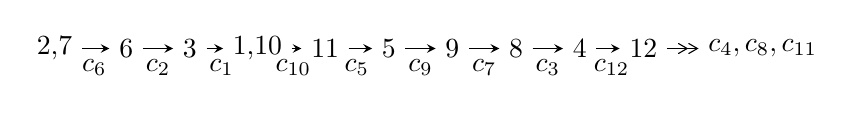
\begin{tikzpicture}[x=23pt, y=7pt]
	% node
	\node (A0) at (-1/8, 0) {2,7};
	\node (A1) at (1, 0) {6};
	\node (A2) at (2, 0) {3};
	\node (A3) at (49/16, 0) {1,10};
	\node (A4) at (33/8, 0) {11};
	\node (A5) at (41/8, 0) {5};
	\node (A6) at (49/8, 0) {9};
	\node (A7) at (57/8, 0) {8};
	\node (A8) at (65/8, 0) {4};
	\node (A9) at (73/8, 0) {12};
	\node (C1) at (1/2, -1) {$c_{6}$};
	\node (C2) at (3/2, -1) {$c_{2}$};
	\node (C3) at (5/2, -1) {$c_{1}$};
	\node (C4) at (29/8, -1) {$c_{10}$};
	\node (C5) at (37/8, -1) {$c_{5}$};
	\node (C6) at (45/8, -1) {$c_{9}$};
	\node (C7) at (53/8, -1) {$c_{7}$};
	\node (C8) at (61/8, -1) {$c_{3}$};
	\node (C9) at (69/8, -1) {$c_{12}$};
	\node (A10) at (11, 0) {$c_{4},c_{8},c_{11}$};

	% edge
	\draw[->,>=stealth]	
	(A0) edge (A1) (A1) edge (A2) (A2) edge (A3) (A3) edge (A4) (A4) edge (A5) (A5) edge (A6) (A6) edge (A7) (A7) edge (A8) (A8) edge (A9) ;
	\draw[->>,>={angle 60}]	
	(A9) edge (A10);
\end{tikzpicture} \\ 

\end{tabular} \\

\footnotetext{
The image of knot diagram is generated by the software ``\textbf{Draw programme}" developed by Andrew Bartholomew(\url{http://www.layer8.co.uk/maths/draw/index.htm\#Running-draw}), where we modified some parts for our purpose(\url{https://github.com/CATsTAILs/LinksPainter}).
}\phantom \\ \newline 
\centering \textbf{Ideals for irreducible components\footnotemark of $X_{\text{par}}$} 
 
\begin{align*}
I^u_{1}&=\langle 
-2.78002\times10^{173} u^{104}+5.41973\times10^{173} u^{103}+\cdots+1.18953\times10^{174} b-3.63788\times10^{175},\\
\phantom{I^u_{1}}&\phantom{= \langle  }-9.01231\times10^{174} u^{104}-1.44968\times10^{175} u^{103}+\cdots+5.94763\times10^{174} a+4.58982\times10^{176},\\
\phantom{I^u_{1}}&\phantom{= \langle  }u^{105}+u^{104}+\cdots-125 u-25\rangle \\
I^u_{2}&=\langle 
28 a^5-43 a^4 u+70 a^4-86 a^3 u+36 a^3-27 a^2 u-16 a^2+16 a u+215 b+189 a-114 u-8,\\
\phantom{I^u_{2}}&\phantom{= \langle  }a^6-2 a^5 u+3 a^5-5 a^4 u+a^4-2 a^3 u-3 a^3+2 a^2 u+3 a^2-5 a u+5 a-3 u+4,\;u^2+1\rangle \\
\\
\end{align*}
\raggedright * 2 irreducible components of $\dim_{\mathbb{C}}=0$, with total 117 representations.\\
\footnotetext{All coefficients of polynomials are rational numbers. But the coefficients are sometimes approximated in decimal forms when there is not enough margin.}
\newpage
\renewcommand{\arraystretch}{1}
\centering \section*{I. $I^u_{1}= \langle -2.78\times10^{173} u^{104}+5.42\times10^{173} u^{103}+\cdots+1.19\times10^{174} b-3.64\times10^{175},\;-9.01\times10^{174} u^{104}-1.45\times10^{175} u^{103}+\cdots+5.95\times10^{174} a+4.59\times10^{176},\;u^{105}+u^{104}+\cdots-125 u-25 \rangle$}
\flushleft \textbf{(i) Arc colorings}\\
\begin{tabular}{m{7pt} m{180pt} m{7pt} m{180pt} }
\flushright $a_{2}=$&$\begin{pmatrix}0\\u\end{pmatrix}$ \\
\flushright $a_{7}=$&$\begin{pmatrix}1\\0\end{pmatrix}$ \\
\flushright $a_{6}=$&$\begin{pmatrix}1\\u^2\end{pmatrix}$ \\
\flushright $a_{3}=$&$\begin{pmatrix}u\\u^3+u\end{pmatrix}$ \\
\flushright $a_{1}=$&$\begin{pmatrix}u^3\\u^5+u^3+u\end{pmatrix}$ \\
\flushright $a_{10}=$&$\begin{pmatrix}1.51528 u^{104}+2.43741 u^{103}+\cdots-342.962 u-77.1705\\0.233708 u^{104}-0.455620 u^{103}+\cdots+106.022 u+30.5826\end{pmatrix}$ \\
\flushright $a_{11}=$&$\begin{pmatrix}1.41422 u^{104}+3.00688 u^{103}+\cdots-376.935 u-86.2579\\-0.102232 u^{104}-0.503588 u^{103}+\cdots+107.840 u+27.3085\end{pmatrix}$ \\
\flushright $a_{5}=$&$\begin{pmatrix}0.107162 u^{104}+0.439090 u^{103}+\cdots-68.2154 u-12.9715\\-1.66904 u^{104}-0.358595 u^{103}+\cdots+71.3230 u+2.74449\end{pmatrix}$ \\
\flushright $a_{9}=$&$\begin{pmatrix}1.74898 u^{104}+1.98179 u^{103}+\cdots-236.940 u-46.5879\\0.233708 u^{104}-0.455620 u^{103}+\cdots+106.022 u+30.5826\end{pmatrix}$ \\
\flushright $a_{8}=$&$\begin{pmatrix}0.0840748 u^{104}+0.942451 u^{103}+\cdots-98.0344 u-26.0878\\0.100962 u^{104}-0.744433 u^{103}+\cdots+141.226 u+39.8498\end{pmatrix}$ \\
\flushright $a_{4}=$&$\begin{pmatrix}-0.990500 u^{104}-3.18401 u^{103}+\cdots+407.098 u+90.6155\\2.57023 u^{104}+0.861705 u^{103}+\cdots-126.916 u-11.1131\end{pmatrix}$ \\
\flushright $a_{12}=$&$\begin{pmatrix}0.301371 u^{104}+2.46302 u^{103}+\cdots-344.399 u-88.0238\\-1.21240 u^{104}-0.508503 u^{103}+\cdots+118.564 u+20.5025\end{pmatrix}$\\&\end{tabular}
\flushleft \textbf{(ii) Obstruction class $= -1$}\\~\\
\flushleft \textbf{(iii) Cusp Shapes $= -3.34744 u^{104}-4.63397 u^{103}+\cdots+773.517 u+167.231$}\\~\\
\newpage\renewcommand{\arraystretch}{1}
\flushleft \textbf{(iv) u-Polynomials at the component}\newline \\
\begin{tabular}{m{50pt}|m{274pt}}
Crossings & \hspace{64pt}u-Polynomials at each crossing \\
\hline $$\begin{aligned}c_{1}\end{aligned}$$&$\begin{aligned}
&u^{105}+51 u^{104}+\cdots-1225 u-625
\end{aligned}$\\
\hline $$\begin{aligned}c_{2},c_{6}\end{aligned}$$&$\begin{aligned}
&u^{105}- u^{104}+\cdots-125 u+25
\end{aligned}$\\
\hline $$\begin{aligned}c_{3},c_{8}\end{aligned}$$&$\begin{aligned}
&u^{105}- u^{104}+\cdots+9 u+1
\end{aligned}$\\
\hline $$\begin{aligned}c_{4},c_{11}\end{aligned}$$&$\begin{aligned}
&u^{105}+u^{104}+\cdots-7 u+1
\end{aligned}$\\
\hline $$\begin{aligned}c_{5}\end{aligned}$$&$\begin{aligned}
&u^{105}-5 u^{104}+\cdots-422719 u+60663
\end{aligned}$\\
\hline $$\begin{aligned}c_{7},c_{9}\end{aligned}$$&$\begin{aligned}
&u^{105}+35 u^{104}+\cdots-43 u+1
\end{aligned}$\\
\hline $$\begin{aligned}c_{10},c_{12}\end{aligned}$$&$\begin{aligned}
&u^{105}-35 u^{104}+\cdots+39 u+1
\end{aligned}$\\
\hline
\end{tabular}\\~\\
\newpage\renewcommand{\arraystretch}{1}
\flushleft \textbf{(v) Riley Polynomials at the component}\newline \\
\begin{tabular}{m{50pt}|m{274pt}}
Crossings & \hspace{64pt}Riley Polynomials at each crossing \\
\hline $$\begin{aligned}c_{1}\end{aligned}$$&$\begin{aligned}
&y^{105}+19 y^{104}+\cdots+36351875 y-390625
\end{aligned}$\\
\hline $$\begin{aligned}c_{2},c_{6}\end{aligned}$$&$\begin{aligned}
&y^{105}+51 y^{104}+\cdots-1225 y-625
\end{aligned}$\\
\hline $$\begin{aligned}c_{3},c_{8}\end{aligned}$$&$\begin{aligned}
&y^{105}-35 y^{104}+\cdots-43 y-1
\end{aligned}$\\
\hline $$\begin{aligned}c_{4},c_{11}\end{aligned}$$&$\begin{aligned}
&y^{105}+35 y^{104}+\cdots+39 y-1
\end{aligned}$\\
\hline $$\begin{aligned}c_{5}\end{aligned}$$&$\begin{aligned}
&y^{105}+15 y^{104}+\cdots+108021991111 y-3679999569
\end{aligned}$\\
\hline $$\begin{aligned}c_{7},c_{9}\end{aligned}$$&$\begin{aligned}
&y^{105}+77 y^{104}+\cdots-5759 y-1
\end{aligned}$\\
\hline $$\begin{aligned}c_{10},c_{12}\end{aligned}$$&$\begin{aligned}
&y^{105}+75 y^{104}+\cdots+951 y-1
\end{aligned}$\\
\hline
\end{tabular}\\~\\
\newpage\flushleft \textbf{(vi) Complex Volumes and Cusp Shapes}
$$\begin{array}{c|c|c}  
\text{Solutions to }I^u_{1}& \I (\text{vol} + \sqrt{-1}CS) & \text{Cusp shape}\\
 \hline 
\begin{aligned}
u &= -0.749218 + 0.639499 I \\
a &= -0.154405 + 0.543190 I \\
b &= \phantom{-}0.077141 + 1.283560 I\end{aligned}
 & \phantom{-}3.66490 - 2.51476 I & \phantom{-0.000000 } 0 \\ \hline\begin{aligned}
u &= -0.749218 - 0.639499 I \\
a &= -0.154405 - 0.543190 I \\
b &= \phantom{-}0.077141 - 1.283560 I\end{aligned}
 & \phantom{-}3.66490 + 2.51476 I & \phantom{-0.000000 } 0 \\ \hline\begin{aligned}
u &= -0.948983 + 0.361206 I \\
a &= -0.206223 - 0.158334 I \\
b &= \phantom{-}0.45260 - 1.51018 I\end{aligned}
 & \phantom{-}2.91142 + 11.55500 I & \phantom{-0.000000 } 0 \\ \hline\begin{aligned}
u &= -0.948983 - 0.361206 I \\
a &= -0.206223 + 0.158334 I \\
b &= \phantom{-}0.45260 + 1.51018 I\end{aligned}
 & \phantom{-}2.91142 - 11.55500 I & \phantom{-0.000000 } 0 \\ \hline\begin{aligned}
u &= \phantom{-}0.922665 + 0.425326 I \\
a &= \phantom{-}0.413418 - 0.143561 I \\
b &= -0.183481 - 1.219410 I\end{aligned}
 & \phantom{-}3.78039 - 5.61089 I & \phantom{-0.000000 } 0 \\ \hline\begin{aligned}
u &= \phantom{-}0.922665 - 0.425326 I \\
a &= \phantom{-}0.413418 + 0.143561 I \\
b &= -0.183481 + 1.219410 I\end{aligned}
 & \phantom{-}3.78039 + 5.61089 I & \phantom{-0.000000 } 0 \\ \hline\begin{aligned}
u &= -0.455269 + 0.915131 I \\
a &= -1.78391 + 1.38691 I \\
b &= \phantom{-}0.417127 + 1.242680 I\end{aligned}
 & -3.63933 - 1.37243 I & \phantom{-0.000000 } 0 \\ \hline\begin{aligned}
u &= -0.455269 - 0.915131 I \\
a &= -1.78391 - 1.38691 I \\
b &= \phantom{-}0.417127 - 1.242680 I\end{aligned}
 & -3.63933 + 1.37243 I & \phantom{-0.000000 } 0 \\ \hline\begin{aligned}
u &= \phantom{-}0.613086 + 0.826892 I \\
a &= \phantom{-}1.021720 + 0.354723 I \\
b &= -0.497693 - 0.157462 I\end{aligned}
 & \phantom{-}3.75864 + 2.41481 I & \phantom{-0.000000 } 0 \\ \hline\begin{aligned}
u &= \phantom{-}0.613086 - 0.826892 I \\
a &= \phantom{-}1.021720 - 0.354723 I \\
b &= -0.497693 + 0.157462 I\end{aligned}
 & \phantom{-}3.75864 - 2.41481 I & \phantom{-0.000000 } 0\\
 \hline 
 \end{array}$$\newpage$$\begin{array}{c|c|c}  
\text{Solutions to }I^u_{1}& \I (\text{vol} + \sqrt{-1}CS) & \text{Cusp shape}\\
 \hline 
\begin{aligned}
u &= \phantom{-}0.896671 + 0.356964 I \\
a &= -0.203981 + 0.291029 I \\
b &= \phantom{-}0.44898 + 1.46429 I\end{aligned}
 & \phantom{-}1.72233 - 5.88113 I & \phantom{-0.000000 } 0 \\ \hline\begin{aligned}
u &= \phantom{-}0.896671 - 0.356964 I \\
a &= -0.203981 - 0.291029 I \\
b &= \phantom{-}0.44898 - 1.46429 I\end{aligned}
 & \phantom{-}1.72233 + 5.88113 I & \phantom{-0.000000 } 0 \\ \hline\begin{aligned}
u &= -0.914248 + 0.490333 I \\
a &= \phantom{-}0.128466 - 0.189595 I \\
b &= \phantom{-}0.33402 - 1.49335 I\end{aligned}
 & \phantom{-}7.99889 + 5.30446 I & \phantom{-0.000000 } 0 \\ \hline\begin{aligned}
u &= -0.914248 - 0.490333 I \\
a &= \phantom{-}0.128466 + 0.189595 I \\
b &= \phantom{-}0.33402 + 1.49335 I\end{aligned}
 & \phantom{-}7.99889 - 5.30446 I & \phantom{-0.000000 } 0 \\ \hline\begin{aligned}
u &= \phantom{-}0.099289 + 1.032690 I \\
a &= -0.503451 - 1.051430 I \\
b &= \phantom{-}0.537831 + 0.973312 I\end{aligned}
 & -1.75450 - 2.05061 I & \phantom{-0.000000 } 0 \\ \hline\begin{aligned}
u &= \phantom{-}0.099289 - 1.032690 I \\
a &= -0.503451 + 1.051430 I \\
b &= \phantom{-}0.537831 - 0.973312 I\end{aligned}
 & -1.75450 + 2.05061 I & \phantom{-0.000000 } 0 \\ \hline\begin{aligned}
u &= -0.854899 + 0.421450 I \\
a &= \phantom{-}0.425038 + 0.283762 I \\
b &= -0.128597 + 1.177340 I\end{aligned}
 & \phantom{-}2.54200 + 0.06951 I & \phantom{-0.000000 } 0 \\ \hline\begin{aligned}
u &= -0.854899 - 0.421450 I \\
a &= \phantom{-}0.425038 - 0.283762 I \\
b &= -0.128597 - 1.177340 I\end{aligned}
 & \phantom{-}2.54200 - 0.06951 I & \phantom{-0.000000 } 0 \\ \hline\begin{aligned}
u &= -0.031016 + 1.049550 I \\
a &= \phantom{-}1.113560 + 0.088475 I \\
b &= -0.0059743 - 0.0144561 I\end{aligned}
 & -4.65129 - 2.79161 I & \phantom{-0.000000 } 0 \\ \hline\begin{aligned}
u &= -0.031016 - 1.049550 I \\
a &= \phantom{-}1.113560 - 0.088475 I \\
b &= -0.0059743 + 0.0144561 I\end{aligned}
 & -4.65129 + 2.79161 I & \phantom{-0.000000 } 0\\
 \hline 
 \end{array}$$\newpage$$\begin{array}{c|c|c}  
\text{Solutions to }I^u_{1}& \I (\text{vol} + \sqrt{-1}CS) & \text{Cusp shape}\\
 \hline 
\begin{aligned}
u &= \phantom{-}0.889111 + 0.570980 I \\
a &= \phantom{-}0.086184 - 0.189831 I \\
b &= -0.068274 - 1.318180 I\end{aligned}
 & \phantom{-}8.53906 + 0.69544 I & \phantom{-0.000000 } 0 \\ \hline\begin{aligned}
u &= \phantom{-}0.889111 - 0.570980 I \\
a &= \phantom{-}0.086184 + 0.189831 I \\
b &= -0.068274 + 1.318180 I\end{aligned}
 & \phantom{-}8.53906 - 0.69544 I & \phantom{-0.000000 } 0 \\ \hline\begin{aligned}
u &= -0.840055 + 0.645863 I \\
a &= \phantom{-}0.575483 - 0.243329 I \\
b &= \phantom{-}0.19081 - 1.42878 I\end{aligned}
 & \phantom{-}5.26478 - 1.27381 I & \phantom{-0.000000 } 0 \\ \hline\begin{aligned}
u &= -0.840055 - 0.645863 I \\
a &= \phantom{-}0.575483 + 0.243329 I \\
b &= \phantom{-}0.19081 + 1.42878 I\end{aligned}
 & \phantom{-}5.26478 + 1.27381 I & \phantom{-0.000000 } 0 \\ \hline\begin{aligned}
u &= -0.412578 + 0.843978 I \\
a &= \phantom{-}2.05627 - 0.88271 I \\
b &= \phantom{-}0.126633 - 1.017210 I\end{aligned}
 & -3.33038 - 2.22358 I & \phantom{-0.000000 } 0 \\ \hline\begin{aligned}
u &= -0.412578 - 0.843978 I \\
a &= \phantom{-}2.05627 + 0.88271 I \\
b &= \phantom{-}0.126633 + 1.017210 I\end{aligned}
 & -3.33038 + 2.22358 I & \phantom{-0.000000 } 0 \\ \hline\begin{aligned}
u &= \phantom{-}0.774233 + 0.531300 I \\
a &= \phantom{-}0.340368 + 0.531499 I \\
b &= \phantom{-}0.293190 + 1.372850 I\end{aligned}
 & \phantom{-}3.36600 - 3.23323 I & \phantom{-0.000000 } 0 \\ \hline\begin{aligned}
u &= \phantom{-}0.774233 - 0.531300 I \\
a &= \phantom{-}0.340368 - 0.531499 I \\
b &= \phantom{-}0.293190 - 1.372850 I\end{aligned}
 & \phantom{-}3.36600 + 3.23323 I & \phantom{-0.000000 } 0 \\ \hline\begin{aligned}
u &= -0.495537 + 0.944166 I \\
a &= -0.75412 + 1.30512 I \\
b &= \phantom{-}0.899731 - 1.079430 I\end{aligned}
 & -3.30148 - 3.57186 I & \phantom{-0.000000 } 0 \\ \hline\begin{aligned}
u &= -0.495537 - 0.944166 I \\
a &= -0.75412 - 1.30512 I \\
b &= \phantom{-}0.899731 + 1.079430 I\end{aligned}
 & -3.30148 + 3.57186 I & \phantom{-0.000000 } 0\\
 \hline 
 \end{array}$$\newpage$$\begin{array}{c|c|c}  
\text{Solutions to }I^u_{1}& \I (\text{vol} + \sqrt{-1}CS) & \text{Cusp shape}\\
 \hline 
\begin{aligned}
u &= \phantom{-}0.472411 + 0.959035 I \\
a &= -1.94854 - 1.12109 I \\
b &= \phantom{-}0.443886 - 1.273270 I\end{aligned}
 & -3.90875 + 7.44310 I & \phantom{-0.000000 } 0 \\ \hline\begin{aligned}
u &= \phantom{-}0.472411 - 0.959035 I \\
a &= -1.94854 + 1.12109 I \\
b &= \phantom{-}0.443886 + 1.273270 I\end{aligned}
 & -3.90875 - 7.44310 I & \phantom{-0.000000 } 0 \\ \hline\begin{aligned}
u &= -0.265182 + 1.035910 I \\
a &= -0.540567 + 0.578355 I \\
b &= \phantom{-}0.627717 + 0.218999 I\end{aligned}
 & -1.64134 - 0.64025 I & \phantom{-0.000000 } 0 \\ \hline\begin{aligned}
u &= -0.265182 - 1.035910 I \\
a &= -0.540567 - 0.578355 I \\
b &= \phantom{-}0.627717 - 0.218999 I\end{aligned}
 & -1.64134 + 0.64025 I & \phantom{-0.000000 } 0 \\ \hline\begin{aligned}
u &= \phantom{-}0.436930 + 0.990417 I \\
a &= -0.70748 - 1.31204 I \\
b &= \phantom{-}0.833111 + 1.105010 I\end{aligned}
 & -4.03635 - 1.85896 I & \phantom{-0.000000 } 0 \\ \hline\begin{aligned}
u &= \phantom{-}0.436930 - 0.990417 I \\
a &= -0.70748 + 1.31204 I \\
b &= \phantom{-}0.833111 - 1.105010 I\end{aligned}
 & -4.03635 + 1.85896 I & \phantom{-0.000000 } 0 \\ \hline\begin{aligned}
u &= \phantom{-}0.827568 + 0.728196 I \\
a &= -0.360735 - 0.251802 I \\
b &= \phantom{-}0.078908 - 1.395500 I\end{aligned}
 & \phantom{-}5.40630 + 7.26455 I & \phantom{-0.000000 } 0 \\ \hline\begin{aligned}
u &= \phantom{-}0.827568 - 0.728196 I \\
a &= -0.360735 + 0.251802 I \\
b &= \phantom{-}0.078908 + 1.395500 I\end{aligned}
 & \phantom{-}5.40630 - 7.26455 I & \phantom{-0.000000 } 0 \\ \hline\begin{aligned}
u &= \phantom{-}0.408500 + 1.043460 I \\
a &= -1.31979 - 0.57260 I \\
b &= \phantom{-}0.987712 - 0.301187 I\end{aligned}
 & -3.74828 + 3.33003 I & \phantom{-0.000000 } 0 \\ \hline\begin{aligned}
u &= \phantom{-}0.408500 - 1.043460 I \\
a &= -1.31979 + 0.57260 I \\
b &= \phantom{-}0.987712 + 0.301187 I\end{aligned}
 & -3.74828 - 3.33003 I & \phantom{-0.000000 } 0\\
 \hline 
 \end{array}$$\newpage$$\begin{array}{c|c|c}  
\text{Solutions to }I^u_{1}& \I (\text{vol} + \sqrt{-1}CS) & \text{Cusp shape}\\
 \hline 
\begin{aligned}
u &= \phantom{-}0.654211 + 0.587061 I \\
a &= \phantom{-}1.095220 + 0.206022 I \\
b &= -0.467679 + 0.101114 I\end{aligned}
 & \phantom{-}0.36679 - 3.18781 I & \phantom{-0.000000 } 0 \\ \hline\begin{aligned}
u &= \phantom{-}0.654211 - 0.587061 I \\
a &= \phantom{-}1.095220 - 0.206022 I \\
b &= -0.467679 - 0.101114 I\end{aligned}
 & \phantom{-}0.36679 + 3.18781 I & \phantom{-0.000000 } 0 \\ \hline\begin{aligned}
u &= -0.523776 + 0.994154 I \\
a &= -1.58817 + 0.36404 I \\
b &= \phantom{-}1.129100 + 0.462674 I\end{aligned}
 & -0.15746 - 5.39094 I & \phantom{-0.000000 } 0 \\ \hline\begin{aligned}
u &= -0.523776 - 0.994154 I \\
a &= -1.58817 - 0.36404 I \\
b &= \phantom{-}1.129100 - 0.462674 I\end{aligned}
 & -0.15746 + 5.39094 I & \phantom{-0.000000 } 0 \\ \hline\begin{aligned}
u &= \phantom{-}0.391092 + 0.779809 I \\
a &= \phantom{-}1.94937 + 1.22961 I \\
b &= \phantom{-}0.181158 + 1.035310 I\end{aligned}
 & -3.18895 - 3.79634 I & \phantom{-0.000000 } 0 \\ \hline\begin{aligned}
u &= \phantom{-}0.391092 - 0.779809 I \\
a &= \phantom{-}1.94937 - 1.22961 I \\
b &= \phantom{-}0.181158 - 1.035310 I\end{aligned}
 & -3.18895 + 3.79634 I & \phantom{-0.000000 } 0 \\ \hline\begin{aligned}
u &= -0.538943 + 0.992209 I \\
a &= \phantom{-}0.892504 - 0.495752 I \\
b &= -0.440179 + 0.375313 I\end{aligned}
 & -1.80743 - 2.63543 I & \phantom{-0.000000 } 0 \\ \hline\begin{aligned}
u &= -0.538943 - 0.992209 I \\
a &= \phantom{-}0.892504 + 0.495752 I \\
b &= -0.440179 - 0.375313 I\end{aligned}
 & -1.80743 + 2.63543 I & \phantom{-0.000000 } 0 \\ \hline\begin{aligned}
u &= \phantom{-}0.602258 + 0.992368 I \\
a &= \phantom{-}0.967009 + 0.515114 I \\
b &= -0.523841 - 0.361124 I\end{aligned}
 & -0.81304 + 8.09901 I & \phantom{-0.000000 } 0 \\ \hline\begin{aligned}
u &= \phantom{-}0.602258 - 0.992368 I \\
a &= \phantom{-}0.967009 - 0.515114 I \\
b &= -0.523841 + 0.361124 I\end{aligned}
 & -0.81304 - 8.09901 I & \phantom{-0.000000 } 0\\
 \hline 
 \end{array}$$\newpage$$\begin{array}{c|c|c}  
\text{Solutions to }I^u_{1}& \I (\text{vol} + \sqrt{-1}CS) & \text{Cusp shape}\\
 \hline 
\begin{aligned}
u &= -0.435933 + 0.697192 I \\
a &= -1.58393 - 0.14120 I \\
b &= \phantom{-}0.906082 + 0.759162 I\end{aligned}
 & -2.52613 - 0.37000 I & \phantom{-0.000000 } 0 \\ \hline\begin{aligned}
u &= -0.435933 - 0.697192 I \\
a &= -1.58393 + 0.14120 I \\
b &= \phantom{-}0.906082 - 0.759162 I\end{aligned}
 & -2.52613 + 0.37000 I & \phantom{-0.000000 } 0 \\ \hline\begin{aligned}
u &= -0.326926 + 0.753509 I \\
a &= \phantom{-}0.876707 - 0.161992 I \\
b &= -0.208415 + 0.097999 I\end{aligned}
 & -0.358551 - 1.274780 I & \phantom{-0.000000 } 0 \\ \hline\begin{aligned}
u &= -0.326926 - 0.753509 I \\
a &= \phantom{-}0.876707 + 0.161992 I \\
b &= -0.208415 - 0.097999 I\end{aligned}
 & -0.358551 + 1.274780 I & \phantom{-0.000000 } 0 \\ \hline\begin{aligned}
u &= \phantom{-}0.727147 + 0.929674 I \\
a &= \phantom{-}1.332630 + 0.067450 I \\
b &= -0.073439 + 1.279710 I\end{aligned}
 & \phantom{-}4.78389 - 1.49312 I & \phantom{-0.000000 } 0 \\ \hline\begin{aligned}
u &= \phantom{-}0.727147 - 0.929674 I \\
a &= \phantom{-}1.332630 - 0.067450 I \\
b &= -0.073439 - 1.279710 I\end{aligned}
 & \phantom{-}4.78389 + 1.49312 I & \phantom{-0.000000 } 0 \\ \hline\begin{aligned}
u &= -0.642428 + 0.994707 I \\
a &= \phantom{-}1.58181 - 0.06710 I \\
b &= -0.120516 - 1.169660 I\end{aligned}
 & \phantom{-}2.58651 - 2.77147 I & \phantom{-0.000000 } 0 \\ \hline\begin{aligned}
u &= -0.642428 - 0.994707 I \\
a &= \phantom{-}1.58181 + 0.06710 I \\
b &= -0.120516 + 1.169660 I\end{aligned}
 & \phantom{-}2.58651 + 2.77147 I & \phantom{-0.000000 } 0 \\ \hline\begin{aligned}
u &= -0.291339 + 1.147920 I \\
a &= -1.07904 + 1.33880 I \\
b &= \phantom{-}0.880929 - 0.060855 I\end{aligned}
 & -7.29427 + 3.25905 I & \phantom{-0.000000 } 0 \\ \hline\begin{aligned}
u &= -0.291339 - 1.147920 I \\
a &= -1.07904 - 1.33880 I \\
b &= \phantom{-}0.880929 + 0.060855 I\end{aligned}
 & -7.29427 - 3.25905 I & \phantom{-0.000000 } 0\\
 \hline 
 \end{array}$$\newpage$$\begin{array}{c|c|c}  
\text{Solutions to }I^u_{1}& \I (\text{vol} + \sqrt{-1}CS) & \text{Cusp shape}\\
 \hline 
\begin{aligned}
u &= \phantom{-}0.318480 + 1.149160 I \\
a &= -1.20502 - 1.21024 I \\
b &= \phantom{-}0.937266 + 0.014042 I\end{aligned}
 & -7.80378 + 2.53380 I & \phantom{-0.000000 } 0 \\ \hline\begin{aligned}
u &= \phantom{-}0.318480 - 1.149160 I \\
a &= -1.20502 + 1.21024 I \\
b &= \phantom{-}0.937266 - 0.014042 I\end{aligned}
 & -7.80378 - 2.53380 I & \phantom{-0.000000 } 0 \\ \hline\begin{aligned}
u &= -0.394685 + 0.681817 I \\
a &= -0.74179 + 1.24370 I \\
b &= \phantom{-}0.858018 - 0.849099 I\end{aligned}
 & \phantom{-}1.00451 + 1.38416 I & \phantom{-0.000000 } 0 \\ \hline\begin{aligned}
u &= -0.394685 - 0.681817 I \\
a &= -0.74179 - 1.24370 I \\
b &= \phantom{-}0.858018 + 0.849099 I\end{aligned}
 & \phantom{-}1.00451 - 1.38416 I & \phantom{-0.000000 } 0 \\ \hline\begin{aligned}
u &= -0.696432 + 0.998477 I \\
a &= -1.363000 + 0.182789 I \\
b &= \phantom{-}0.36242 + 1.47257 I\end{aligned}
 & \phantom{-}4.19020 - 4.43268 I & \phantom{-0.000000 } 0 \\ \hline\begin{aligned}
u &= -0.696432 - 0.998477 I \\
a &= -1.363000 - 0.182789 I \\
b &= \phantom{-}0.36242 - 1.47257 I\end{aligned}
 & \phantom{-}4.19020 + 4.43268 I & \phantom{-0.000000 } 0 \\ \hline\begin{aligned}
u &= \phantom{-}0.525892 + 1.105600 I \\
a &= -1.70195 - 0.58889 I \\
b &= \phantom{-}1.227660 - 0.311645 I\end{aligned}
 & -6.36079 + 5.15428 I & \phantom{-0.000000 } 0 \\ \hline\begin{aligned}
u &= \phantom{-}0.525892 - 1.105600 I \\
a &= -1.70195 + 0.58889 I \\
b &= \phantom{-}1.227660 + 0.311645 I\end{aligned}
 & -6.36079 - 5.15428 I & \phantom{-0.000000 } 0 \\ \hline\begin{aligned}
u &= -0.557253 + 1.100040 I \\
a &= -1.75299 + 0.53655 I \\
b &= \phantom{-}1.264240 + 0.349874 I\end{aligned}
 & -5.43018 - 10.86880 I & \phantom{-0.000000 } 0 \\ \hline\begin{aligned}
u &= -0.557253 - 1.100040 I \\
a &= -1.75299 - 0.53655 I \\
b &= \phantom{-}1.264240 - 0.349874 I\end{aligned}
 & -5.43018 + 10.86880 I & \phantom{-0.000000 } 0\\
 \hline 
 \end{array}$$\newpage$$\begin{array}{c|c|c}  
\text{Solutions to }I^u_{1}& \I (\text{vol} + \sqrt{-1}CS) & \text{Cusp shape}\\
 \hline 
\begin{aligned}
u &= \phantom{-}0.633066 + 1.062180 I \\
a &= -1.71464 - 0.17211 I \\
b &= \phantom{-}0.45172 - 1.45583 I\end{aligned}
 & \phantom{-}1.76945 + 8.55794 I & \phantom{-0.000000 } 0 \\ \hline\begin{aligned}
u &= \phantom{-}0.633066 - 1.062180 I \\
a &= -1.71464 + 0.17211 I \\
b &= \phantom{-}0.45172 + 1.45583 I\end{aligned}
 & \phantom{-}1.76945 - 8.55794 I & \phantom{-0.000000 } 0 \\ \hline\begin{aligned}
u &= -0.157329 + 1.256680 I \\
a &= \phantom{-}0.153650 - 1.003600 I \\
b &= \phantom{-}0.055397 + 0.979337 I\end{aligned}
 & -3.05816 - 2.74237 I & \phantom{-0.000000 } 0 \\ \hline\begin{aligned}
u &= -0.157329 - 1.256680 I \\
a &= \phantom{-}0.153650 + 1.003600 I \\
b &= \phantom{-}0.055397 - 0.979337 I\end{aligned}
 & -3.05816 + 2.74237 I & \phantom{-0.000000 } 0 \\ \hline\begin{aligned}
u &= -0.659194 + 0.320658 I \\
a &= -0.514042 + 0.767799 I \\
b &= \phantom{-}1.036400 - 0.466896 I\end{aligned}
 & -3.24371 + 6.12777 I & -6.15771 - 5.80608 I \\ \hline\begin{aligned}
u &= -0.659194 - 0.320658 I \\
a &= -0.514042 - 0.767799 I \\
b &= \phantom{-}1.036400 + 0.466896 I\end{aligned}
 & -3.24371 - 6.12777 I & -6.15771 + 5.80608 I \\ \hline\begin{aligned}
u &= \phantom{-}0.705819 + 1.068090 I \\
a &= \phantom{-}1.55412 - 0.13299 I \\
b &= -0.223821 + 1.220860 I\end{aligned}
 & \phantom{-}7.02983 + 5.17717 I & \phantom{-0.000000 } 0 \\ \hline\begin{aligned}
u &= \phantom{-}0.705819 - 1.068090 I \\
a &= \phantom{-}1.55412 + 0.13299 I \\
b &= -0.223821 - 1.220860 I\end{aligned}
 & \phantom{-}7.02983 - 5.17717 I & \phantom{-0.000000 } 0 \\ \hline\begin{aligned}
u &= -0.638249 + 1.127680 I \\
a &= \phantom{-}1.71290 + 0.16233 I \\
b &= -0.276567 - 1.120920 I\end{aligned}
 & \phantom{-}0.42944 - 5.60887 I & \phantom{-0.000000 } 0 \\ \hline\begin{aligned}
u &= -0.638249 - 1.127680 I \\
a &= \phantom{-}1.71290 - 0.16233 I \\
b &= -0.276567 + 1.120920 I\end{aligned}
 & \phantom{-}0.42944 + 5.60887 I & \phantom{-0.000000 } 0\\
 \hline 
 \end{array}$$\newpage$$\begin{array}{c|c|c}  
\text{Solutions to }I^u_{1}& \I (\text{vol} + \sqrt{-1}CS) & \text{Cusp shape}\\
 \hline 
\begin{aligned}
u &= \phantom{-}0.208539 + 1.286940 I \\
a &= -0.33208 - 1.39539 I \\
b &= \phantom{-}0.471474 + 1.286510 I\end{aligned}
 & -3.77595 - 2.49413 I & \phantom{-0.000000 } 0 \\ \hline\begin{aligned}
u &= \phantom{-}0.208539 - 1.286940 I \\
a &= -0.33208 + 1.39539 I \\
b &= \phantom{-}0.471474 - 1.286510 I\end{aligned}
 & -3.77595 + 2.49413 I & \phantom{-0.000000 } 0 \\ \hline\begin{aligned}
u &= \phantom{-}0.652851 + 0.229553 I \\
a &= -0.391974 - 0.605737 I \\
b &= \phantom{-}1.000530 + 0.352950 I\end{aligned}
 & -3.94841 - 0.62805 I & -8.02207 + 0.40086 I \\ \hline\begin{aligned}
u &= \phantom{-}0.652851 - 0.229553 I \\
a &= -0.391974 + 0.605737 I \\
b &= \phantom{-}1.000530 - 0.352950 I\end{aligned}
 & -3.94841 + 0.62805 I & -8.02207 - 0.40086 I \\ \hline\begin{aligned}
u &= -0.045533 + 1.308020 I \\
a &= -0.118848 + 1.278670 I \\
b &= \phantom{-}0.274612 - 1.204280 I\end{aligned}
 & \phantom{-}1.44896 + 2.66591 I & \phantom{-0.000000 } 0 \\ \hline\begin{aligned}
u &= -0.045533 - 1.308020 I \\
a &= -0.118848 - 1.278670 I \\
b &= \phantom{-}0.274612 + 1.204280 I\end{aligned}
 & \phantom{-}1.44896 - 2.66591 I & \phantom{-0.000000 } 0 \\ \hline\begin{aligned}
u &= -0.545403 + 0.420809 I \\
a &= \phantom{-}1.077950 - 0.122804 I \\
b &= -0.300695 - 0.199395 I\end{aligned}
 & -0.34516 - 1.69194 I & -0.65997 + 3.30204 I \\ \hline\begin{aligned}
u &= -0.545403 - 0.420809 I \\
a &= \phantom{-}1.077950 + 0.122804 I \\
b &= -0.300695 + 0.199395 I\end{aligned}
 & -0.34516 + 1.69194 I & -0.65997 - 3.30204 I \\ \hline\begin{aligned}
u &= -0.684533 + 1.119160 I \\
a &= -1.68900 - 0.11987 I \\
b &= \phantom{-}0.47230 + 1.53335 I\end{aligned}
 & \phantom{-}6.08933 - 11.17010 I & \phantom{-0.000000 } 0 \\ \hline\begin{aligned}
u &= -0.684533 - 1.119160 I \\
a &= -1.68900 + 0.11987 I \\
b &= \phantom{-}0.47230 - 1.53335 I\end{aligned}
 & \phantom{-}6.08933 + 11.17010 I & \phantom{-0.000000 } 0\\
 \hline 
 \end{array}$$\newpage$$\begin{array}{c|c|c}  
\text{Solutions to }I^u_{1}& \I (\text{vol} + \sqrt{-1}CS) & \text{Cusp shape}\\
 \hline 
\begin{aligned}
u &= \phantom{-}0.119068 + 1.317990 I \\
a &= \phantom{-}0.138283 + 1.145170 I \\
b &= \phantom{-}0.060042 - 1.094540 I\end{aligned}
 & -2.36377 - 2.50056 I & \phantom{-0.000000 } 0 \\ \hline\begin{aligned}
u &= \phantom{-}0.119068 - 1.317990 I \\
a &= \phantom{-}0.138283 - 1.145170 I \\
b &= \phantom{-}0.060042 + 1.094540 I\end{aligned}
 & -2.36377 + 2.50056 I & \phantom{-0.000000 } 0 \\ \hline\begin{aligned}
u &= \phantom{-}0.628153 + 1.166960 I \\
a &= -1.95577 + 0.16084 I \\
b &= \phantom{-}0.54821 - 1.50960 I\end{aligned}
 & -0.71454 + 11.48410 I & \phantom{-0.000000 } 0 \\ \hline\begin{aligned}
u &= \phantom{-}0.628153 - 1.166960 I \\
a &= -1.95577 - 0.16084 I \\
b &= \phantom{-}0.54821 + 1.50960 I\end{aligned}
 & -0.71454 - 11.48410 I & \phantom{-0.000000 } 0 \\ \hline\begin{aligned}
u &= \phantom{-}0.661390 + 1.149150 I \\
a &= \phantom{-}1.69582 - 0.21098 I \\
b &= -0.310769 + 1.143510 I\end{aligned}
 & \phantom{-}1.58523 + 11.41040 I & \phantom{-0.000000 } 0 \\ \hline\begin{aligned}
u &= \phantom{-}0.661390 - 1.149150 I \\
a &= \phantom{-}1.69582 + 0.21098 I \\
b &= -0.310769 - 1.143510 I\end{aligned}
 & \phantom{-}1.58523 - 11.41040 I & \phantom{-0.000000 } 0 \\ \hline\begin{aligned}
u &= -0.186843 + 1.334870 I \\
a &= -0.27019 + 1.43191 I \\
b &= \phantom{-}0.419159 - 1.326740 I\end{aligned}
 & -2.94616 + 7.93415 I & \phantom{-0.000000 } 0 \\ \hline\begin{aligned}
u &= -0.186843 - 1.334870 I \\
a &= -0.27019 - 1.43191 I \\
b &= \phantom{-}0.419159 + 1.326740 I\end{aligned}
 & -2.94616 - 7.93415 I & \phantom{-0.000000 } 0 \\ \hline\begin{aligned}
u &= -0.644955 + 1.184790 I \\
a &= -1.93120 - 0.24671 I \\
b &= \phantom{-}0.55527 + 1.53543 I\end{aligned}
 & \phantom{-}0.4062 - 17.3601 I & \phantom{-0.000000 } 0 \\ \hline\begin{aligned}
u &= -0.644955 - 1.184790 I \\
a &= -1.93120 + 0.24671 I \\
b &= \phantom{-}0.55527 - 1.53543 I\end{aligned}
 & \phantom{-}0.4062 + 17.3601 I & \phantom{-0.000000 } 0\\
 \hline 
 \end{array}$$\newpage$$\begin{array}{c|c|c}  
\text{Solutions to }I^u_{1}& \I (\text{vol} + \sqrt{-1}CS) & \text{Cusp shape}\\
 \hline 
\begin{aligned}
u &= \phantom{-}0.369462 + 0.499023 I \\
a &= -1.88737 + 0.31530 I \\
b &= \phantom{-}0.810482 - 0.869250 I\end{aligned}
 & -2.57683 + 5.38819 I & -4.57971 - 8.38711 I \\ \hline\begin{aligned}
u &= \phantom{-}0.369462 - 0.499023 I \\
a &= -1.88737 - 0.31530 I \\
b &= \phantom{-}0.810482 + 0.869250 I\end{aligned}
 & -2.57683 - 5.38819 I & -4.57971 + 8.38711 I \\ \hline\begin{aligned}
u &= \phantom{-}0.481861\phantom{ +0.000000I} \\
a &= \phantom{-}0.400491\phantom{ +0.000000I} \\
b &= \phantom{-}0.607759\phantom{ +0.000000I}\end{aligned}
 & -1.15266\phantom{ +0.000000I} & -8.89830\phantom{ +0.000000I} \\ \hline\begin{aligned}
u &= -0.342083 + 0.052573 I \\
a &= \phantom{-}1.61547 + 0.81293 I \\
b &= \phantom{-}0.374191 - 0.564968 I\end{aligned}
 & \phantom{-}1.25400 + 1.74865 I & \phantom{-}2.56111 - 5.04515 I \\ \hline\begin{aligned}
u &= -0.342083 - 0.052573 I \\
a &= \phantom{-}1.61547 - 0.81293 I \\
b &= \phantom{-}0.374191 + 0.564968 I\end{aligned}
 & \phantom{-}1.25400 - 1.74865 I & \phantom{-}2.56111 + 5.04515 I\\
 \hline 
 \end{array}$$\newpage\newpage\renewcommand{\arraystretch}{1}
\centering \section*{II. $I^u_{2}= \langle -43 a^4 u-86 a^3 u+\cdots+189 a-8,\;-2 a^5 u-5 a^4 u+\cdots+5 a+4,\;u^2+1 \rangle$}
\flushleft \textbf{(i) Arc colorings}\\
\begin{tabular}{m{7pt} m{180pt} m{7pt} m{180pt} }
\flushright $a_{2}=$&$\begin{pmatrix}0\\u\end{pmatrix}$ \\
\flushright $a_{7}=$&$\begin{pmatrix}1\\0\end{pmatrix}$ \\
\flushright $a_{6}=$&$\begin{pmatrix}1\\-1\end{pmatrix}$ \\
\flushright $a_{3}=$&$\begin{pmatrix}u\\0\end{pmatrix}$ \\
\flushright $a_{1}=$&$\begin{pmatrix}- u\\u\end{pmatrix}$ \\
\flushright $a_{10}=$&$\begin{pmatrix}a\\0.200000 a^{4} u+0.400000 a^{3} u+\cdots-0.879070 a+0.0372093\end{pmatrix}$ \\
\flushright $a_{11}=$&$\begin{pmatrix}-0.200000 a^{4} u-0.400000 a^{3} u+\cdots+0.879070 a-0.0372093\\0.400000 a^{4} u+0.800000 a^{3} u+\cdots-0.758140 a+0.0744186\end{pmatrix}$ \\
\flushright $a_{5}=$&$\begin{pmatrix}0.0604651 a^{5} u+0.251163 a^{4} u+\cdots-0.688372 a+0.479070\\0.0604651 a^{5} u+0.0511628 a^{4} u+\cdots+0.190698 a-0.558140\end{pmatrix}$ \\
\flushright $a_{9}=$&$\begin{pmatrix}0.200000 a^{4} u+0.400000 a^{3} u+\cdots+0.120930 a+0.0372093\\0.200000 a^{4} u+0.400000 a^{3} u+\cdots-0.879070 a+0.0372093\end{pmatrix}$ \\
\flushright $a_{8}=$&$\begin{pmatrix}-0.0604651 a^{5} u-0.0511628 a^{4} u+\cdots-0.190698 a+0.558140\\0.200000 a^{4} u+0.400000 a^{3} u+\cdots-0.879070 a-0.962791\end{pmatrix}$ \\
\flushright $a_{4}=$&$\begin{pmatrix}- a u\\0.130233 a^{5} u+0.325581 a^{4} u+\cdots-0.0744186 a+0.530233\end{pmatrix}$ \\
\flushright $a_{12}=$&$\begin{pmatrix}-0.0651163 a^{5} u-0.362791 a^{4} u+\cdots+0.195349 a-0.139535\\0.0651163 a^{5} u+0.762791 a^{4} u+\cdots-0.511628 a-0.111628\end{pmatrix}$\\&\end{tabular}
\flushleft \textbf{(ii) Obstruction class $= 1$}\\~\\
\flushleft \textbf{(iii) Cusp Shapes $= -\frac{8}{215} a^5 u-\frac{112}{215} a^5+\frac{152}{215} a^4 u-\frac{108}{215} a^4+\frac{88}{215} a^3 u+\frac{40}{43} a^3-\frac{256}{215} a^2 u-\frac{128}{215} a^2+\frac{312}{215} a u-\frac{224}{43} a+\frac{704}{215} u-\frac{1352}{215}$}\\~\\
\newpage\renewcommand{\arraystretch}{1}
\flushleft \textbf{(iv) u-Polynomials at the component}\newline \\
\begin{tabular}{m{50pt}|m{274pt}}
Crossings & \hspace{64pt}u-Polynomials at each crossing \\
\hline $$\begin{aligned}c_{1}\end{aligned}$$&$\begin{aligned}
&(u-1)^{12}
\end{aligned}$\\
\hline $$\begin{aligned}c_{2},c_{6}\end{aligned}$$&$\begin{aligned}
&(u^2+1)^6
\end{aligned}$\\
\hline $$\begin{aligned}c_{3},c_{8}\end{aligned}$$&$\begin{aligned}
&(u^4- u^2+1)^3
\end{aligned}$\\
\hline $$\begin{aligned}c_{4},c_{11}\end{aligned}$$&$\begin{aligned}
&(u^6+u^4+2 u^2+1)^2
\end{aligned}$\\
\hline $$\begin{aligned}c_{5}\end{aligned}$$&$\begin{aligned}
&(u^6-3 u^4+2 u^2+1)^2
\end{aligned}$\\
\hline $$\begin{aligned}c_{7}\end{aligned}$$&$\begin{aligned}
&(u^2- u+1)^6
\end{aligned}$\\
\hline $$\begin{aligned}c_{9}\end{aligned}$$&$\begin{aligned}
&(u^2+u+1)^6
\end{aligned}$\\
\hline $$\begin{aligned}c_{10}\end{aligned}$$&$\begin{aligned}
&(u^3+u^2+2 u+1)^4
\end{aligned}$\\
\hline $$\begin{aligned}c_{12}\end{aligned}$$&$\begin{aligned}
&(u^3- u^2+2 u-1)^4
\end{aligned}$\\
\hline
\end{tabular}\\~\\
\newpage\renewcommand{\arraystretch}{1}
\flushleft \textbf{(v) Riley Polynomials at the component}\newline \\
\begin{tabular}{m{50pt}|m{274pt}}
Crossings & \hspace{64pt}Riley Polynomials at each crossing \\
\hline $$\begin{aligned}c_{1}\end{aligned}$$&$\begin{aligned}
&(y-1)^{12}
\end{aligned}$\\
\hline $$\begin{aligned}c_{2},c_{6}\end{aligned}$$&$\begin{aligned}
&(y+1)^{12}
\end{aligned}$\\
\hline $$\begin{aligned}c_{3},c_{8}\end{aligned}$$&$\begin{aligned}
&(y^2- y+1)^6
\end{aligned}$\\
\hline $$\begin{aligned}c_{4},c_{11}\end{aligned}$$&$\begin{aligned}
&(y^3+y^2+2 y+1)^4
\end{aligned}$\\
\hline $$\begin{aligned}c_{5}\end{aligned}$$&$\begin{aligned}
&(y^3-3 y^2+2 y+1)^4
\end{aligned}$\\
\hline $$\begin{aligned}c_{7},c_{9}\end{aligned}$$&$\begin{aligned}
&(y^2+y+1)^6
\end{aligned}$\\
\hline $$\begin{aligned}c_{10},c_{12}\end{aligned}$$&$\begin{aligned}
&(y^3+3 y^2+2 y-1)^4
\end{aligned}$\\
\hline
\end{tabular}\\~\\
\newpage\flushleft \textbf{(vi) Complex Volumes and Cusp Shapes}
$$\begin{array}{c|c|c}  
\text{Solutions to }I^u_{2}& \I (\text{vol} + \sqrt{-1}CS) & \text{Cusp shape}\\
 \hline 
\begin{aligned}
u &= \phantom{-0.000000 -}1.000000 I \\
a &= \phantom{-}0.807141 - 0.650946 I \\
b &= \phantom{-}0.500000 + 0.866025 I\end{aligned}
 & -4.66906 - 4.85801 I & -9.50976 + 6.44355 I \\ \hline\begin{aligned}
u &= \phantom{-0.000000 -}1.000000 I \\
a &= \phantom{-}0.807141 + 1.081110 I \\
b &= \phantom{-}0.500000 - 0.866025 I\end{aligned}
 & -4.66906 - 0.79824 I & -9.50976 - 0.48465 I \\ \hline\begin{aligned}
u &= \phantom{-0.000000 -}1.000000 I \\
a &= -0.500000 - 0.296185 I \\
b &= \phantom{-}0.500000 + 0.866025 I\end{aligned}
 & -0.53148 - 2.02988 I & -2.98049 + 3.46410 I \\ \hline\begin{aligned}
u &= \phantom{-0.000000 -}1.000000 I \\
a &= -0.50000 + 1.43587 I \\
b &= \phantom{-}0.500000 - 0.866025 I\end{aligned}
 & -0.53148 + 2.02988 I & -2.98049 - 3.46410 I \\ \hline\begin{aligned}
u &= \phantom{-0.000000 -}1.000000 I \\
a &= -1.80714 - 0.65095 I \\
b &= \phantom{-}0.500000 + 0.866025 I\end{aligned}
 & -4.66906 + 0.79824 I & -9.50976 + 0.48465 I \\ \hline\begin{aligned}
u &= \phantom{-0.000000 -}1.000000 I \\
a &= -1.80714 + 1.08111 I \\
b &= \phantom{-}0.500000 - 0.866025 I\end{aligned}
 & -4.66906 + 4.85801 I & -9.50976 - 6.44355 I \\ \hline\begin{aligned}
u &= \phantom{-0.000000 } -1.000000 I \\
a &= \phantom{-}0.807141 + 0.650946 I \\
b &= \phantom{-}0.500000 - 0.866025 I\end{aligned}
 & -4.66906 + 4.85801 I & -9.50976 - 6.44355 I \\ \hline\begin{aligned}
u &= \phantom{-0.000000 } -1.000000 I \\
a &= \phantom{-}0.807141 - 1.081110 I \\
b &= \phantom{-}0.500000 + 0.866025 I\end{aligned}
 & -4.66906 + 0.79824 I & -9.50976 + 0.48465 I \\ \hline\begin{aligned}
u &= \phantom{-0.000000 } -1.000000 I \\
a &= -0.500000 + 0.296185 I \\
b &= \phantom{-}0.500000 - 0.866025 I\end{aligned}
 & -0.53148 + 2.02988 I & -2.98049 - 3.46410 I \\ \hline\begin{aligned}
u &= \phantom{-0.000000 } -1.000000 I \\
a &= -0.50000 - 1.43587 I \\
b &= \phantom{-}0.500000 + 0.866025 I\end{aligned}
 & -0.53148 - 2.02988 I & -2.98049 + 3.46410 I\\
 \hline 
 \end{array}$$\newpage$$\begin{array}{c|c|c}  
\text{Solutions to }I^u_{2}& \I (\text{vol} + \sqrt{-1}CS) & \text{Cusp shape}\\
 \hline 
\begin{aligned}
u &= \phantom{-0.000000 } -1.000000 I \\
a &= -1.80714 + 0.65095 I \\
b &= \phantom{-}0.500000 - 0.866025 I\end{aligned}
 & -4.66906 - 0.79824 I & -9.50976 - 0.48465 I \\ \hline\begin{aligned}
u &= \phantom{-0.000000 } -1.000000 I \\
a &= -1.80714 - 1.08111 I \\
b &= \phantom{-}0.500000 + 0.866025 I\end{aligned}
 & -4.66906 - 4.85801 I & -9.50976 + 6.44355 I\\
 \hline 
 \end{array}$$\newpage
\newpage\renewcommand{\arraystretch}{1}
\centering \section*{ III. u-Polynomials}
\begin{tabular}{m{50pt}|m{274pt}}
Crossings & \hspace{64pt}u-Polynomials at each crossing \\
\hline $$\begin{aligned}c_{1}\end{aligned}$$&$\begin{aligned}
&((u-1)^{12})(u^{105}+51 u^{104}+\cdots-1225 u-625)
\end{aligned}$\\
\hline $$\begin{aligned}c_{2},c_{6}\end{aligned}$$&$\begin{aligned}
&((u^2+1)^6)(u^{105}- u^{104}+\cdots-125 u+25)
\end{aligned}$\\
\hline $$\begin{aligned}c_{3},c_{8}\end{aligned}$$&$\begin{aligned}
&((u^4- u^2+1)^3)(u^{105}- u^{104}+\cdots+9 u+1)
\end{aligned}$\\
\hline $$\begin{aligned}c_{4},c_{11}\end{aligned}$$&$\begin{aligned}
&((u^6+u^4+2 u^2+1)^2)(u^{105}+u^{104}+\cdots-7 u+1)
\end{aligned}$\\
\hline $$\begin{aligned}c_{5}\end{aligned}$$&$\begin{aligned}
&((u^6-3 u^4+2 u^2+1)^2)(u^{105}-5 u^{104}+\cdots-422719 u+60663)
\end{aligned}$\\
\hline $$\begin{aligned}c_{7}\end{aligned}$$&$\begin{aligned}
&((u^2- u+1)^6)(u^{105}+35 u^{104}+\cdots-43 u+1)
\end{aligned}$\\
\hline $$\begin{aligned}c_{9}\end{aligned}$$&$\begin{aligned}
&((u^2+u+1)^6)(u^{105}+35 u^{104}+\cdots-43 u+1)
\end{aligned}$\\
\hline $$\begin{aligned}c_{10}\end{aligned}$$&$\begin{aligned}
&((u^3+u^2+2 u+1)^4)(u^{105}-35 u^{104}+\cdots+39 u+1)
\end{aligned}$\\
\hline $$\begin{aligned}c_{12}\end{aligned}$$&$\begin{aligned}
&((u^3- u^2+2 u-1)^4)(u^{105}-35 u^{104}+\cdots+39 u+1)
\end{aligned}$\\
\hline
\end{tabular}\newpage\renewcommand{\arraystretch}{1}
\centering \section*{ IV. Riley Polynomials}
\begin{tabular}{m{50pt}|m{274pt}}
Crossings & \hspace{64pt}Riley Polynomials at each crossing \\
\hline $$\begin{aligned}c_{1}\end{aligned}$$&$\begin{aligned}
&((y-1)^{12})(y^{105}+19 y^{104}+\cdots+3.63519\times10^{7} y-390625)
\end{aligned}$\\
\hline $$\begin{aligned}c_{2},c_{6}\end{aligned}$$&$\begin{aligned}
&((y+1)^{12})(y^{105}+51 y^{104}+\cdots-1225 y-625)
\end{aligned}$\\
\hline $$\begin{aligned}c_{3},c_{8}\end{aligned}$$&$\begin{aligned}
&((y^2- y+1)^6)(y^{105}-35 y^{104}+\cdots-43 y-1)
\end{aligned}$\\
\hline $$\begin{aligned}c_{4},c_{11}\end{aligned}$$&$\begin{aligned}
&((y^3+y^2+2 y+1)^4)(y^{105}+35 y^{104}+\cdots+39 y-1)
\end{aligned}$\\
\hline $$\begin{aligned}c_{5}\end{aligned}$$&$\begin{aligned}
&(y^3-3 y^2+2 y+1)^4\\
&\cdot(y^{105}+15 y^{104}+\cdots+108021991111 y-3679999569)
\end{aligned}$\\
\hline $$\begin{aligned}c_{7},c_{9}\end{aligned}$$&$\begin{aligned}
&((y^2+y+1)^6)(y^{105}+77 y^{104}+\cdots-5759 y-1)
\end{aligned}$\\
\hline $$\begin{aligned}c_{10},c_{12}\end{aligned}$$&$\begin{aligned}
&((y^3+3 y^2+2 y-1)^4)(y^{105}+75 y^{104}+\cdots+951 y-1)
\end{aligned}$\\
\hline
\end{tabular}
\vskip 2pc
\end{document}